\documentclass{beamer}
\usepackage[utf8]{inputenc}
\usepackage{graphicx, epsfig}
\usepackage{amsmath,mathrsfs,amsfonts,amssymb}
\usepackage{floatflt}
\usepackage{epic,ecltree}
\usepackage{mathtext}
\usepackage{fancybox}
\usepackage{fancyhdr}
\usepackage{multirow}
\usepackage{enumerate}
\usepackage{epstopdf}
\usepackage{multicol}
\usepackage{algorithm}
\usepackage[noend]{algorithmic}
\usepackage{tikz}
\usepackage{blindtext}
\usetheme{default}%{Singapore}%{Warsaw}%{Warsaw}%{Darmstadt}
\usecolortheme{default}

\setbeamerfont{title}{size=\Huge}
\setbeamertemplate{footline}[page number]{}

\setbeamertemplate{section in toc}[sections numbered]


\makeatletter
\newcommand\HUGE{\@setfontsize\Huge{35}{40}}
\makeatother    

\setbeamerfont{title}{size=\HUGE}
\beamertemplatenavigationsymbolsempty

% latin bold lower
\newcommand{\ba}{\mathbf{a}} 
\newcommand{\bc}{\mathbf{c}} 
\newcommand{\be}{\mathbf{e}} 
\newcommand{\bff}{\mathbf{f}} % \bf - for bold type
\newcommand{\bg}{\mathbf{g}} 
\newcommand{\bh}{\mathbf{h}} 
\newcommand{\bp}{\mathbf{p}} 
\newcommand{\bq}{\mathbf{q}} 
\newcommand{\bt}{\mathbf{t}} 
\newcommand{\bs}{\mathbf{s}} 
\newcommand{\bu}{\mathbf{u}} 
\newcommand{\bv}{\mathbf{v}} 
\newcommand{\bw}{\mathbf{w}} 
\newcommand{\bx}{\mathbf{x}} 
\newcommand{\by}{\mathbf{y}} 
\newcommand{\bz}{\mathbf{z}} 

% latin bold upper
\newcommand{\bA}{\mathbf{A}} 
\newcommand{\bB}{\mathbf{B}} 
\newcommand{\bC}{\mathbf{C}} 
\newcommand{\bG}{\mathbf{G}} 
\newcommand{\bI}{\mathbf{I}} 
\newcommand{\bJ}{\mathbf{J}} 
\newcommand{\bL}{\mathbf{L}} 
\newcommand{\bM}{\mathbf{M}} 
\newcommand{\bP}{\mathbf{P}}
\newcommand{\bQ}{\mathbf{Q}} 
\newcommand{\bR}{\mathbf{R}} 
\newcommand{\bT}{\mathbf{T}} 
\newcommand{\bU}{\mathbf{U}} 
\newcommand{\bV}{\mathbf{V}} 
\newcommand{\bW}{\mathbf{W}} 
\newcommand{\bX}{\mathbf{X}} 
\newcommand{\bY}{\mathbf{Y}} 
\newcommand{\bZ}{\mathbf{Z}} 

% latin cal upper
\newcommand{\cF}{\mathcal{F}} 
\newcommand{\cG}{\mathcal{G}} 
\newcommand{\cI}{\mathcal{I}} 
\newcommand{\cL}{\mathcal{L}} 
\newcommand{\cM}{\mathcal{M}} 
\newcommand{\cN}{\mathcal{N}} 
\newcommand{\cP}{\mathcal{P}} 
\newcommand{\cS}{\mathcal{S}} 
\newcommand{\cT}{\mathcal{T}} 
\newcommand{\cW}{\mathcal{W}} 
\newcommand{\cX}{\mathcal{X}} 
\newcommand{\cZ}{\mathcal{Z}} 

% latin bb upper
\newcommand{\bbE}{\mathbb{E}} 
\newcommand{\bbI}{\mathbb{I}} 
\newcommand{\bbP}{\mathbb{P}} 
\newcommand{\bbR}{\mathbb{R}} 

% greek bold lower
\newcommand{\bepsilon}{\boldsymbol{\epsilon}} 
\newcommand{\btheta}{\boldsymbol{\theta}} 
\newcommand{\blambda}{\boldsymbol{\lambda}} 
\newcommand{\bpi}{\boldsymbol{\pi}} 
\newcommand{\bmu}{\boldsymbol{\mu}} 
\newcommand{\bsigma}{\boldsymbol{\sigma}} 
\newcommand{\bphi}{\boldsymbol{\phi}} 

% greek bold upper
\newcommand{\bSigma}{\boldsymbol{\Sigma}} 

\DeclareMathOperator*{\argmin}{arg\,min}
\DeclareMathOperator*{\argmax}{arg\,max}

\newcommand{\createdgmtitle}[1]{\title[\hbox to 56mm{Deep Generative Models  \hfill\insertframenumber\,/\,\inserttotalframenumber}]
	{\vspace{1cm} \\ \textbf{Deep Generative Models} \\ {\Huge Lecture #1}}
	\author{Roman Isachenko}
		\institute{
\includegraphics[width=0.7cm]{../utils/aimasterslogo} \LARGE{AI Masters}}
	\date{2024, Summer}
}

\usepackage{tikz}
\usetikzlibrary{arrows,shapes,positioning,shadows,trees}

\newcommand\myfootnote[1]{%
  \tikz[remember picture,overlay]
  \draw (current page.south west) +(1in + \oddsidemargin,0.5em)
  node[anchor=south west,inner sep=0pt]{\parbox{\textwidth}{%
      \rlap{\rule{10em}{0.4pt}}\raggedright\scriptsize \textit{#1}}};}

\newcommand\myfootnotewithlink[2]{%
  \tikz[remember picture,overlay]
  \draw (current page.south west) +(1in + \oddsidemargin,0.5em)
  node[anchor=south west,inner sep=0pt]{\parbox{\textwidth}{%
      \rlap{\rule{10em}{0.4pt}}\raggedright\scriptsize\href{#1}{\textit{#2}}}};}
      
\AtBeginSection[]
      {
      	\begin{frame}{Outline}
      		\tableofcontents[currentsection]
      	\end{frame}
      }
      \AtBeginSubsection[]{
      	\begin{frame}{Outline}
      		\tableofcontents[currentsection,currentsubsection]
      	\end{frame}
}
\createdgmtitle{13}

\usepackage{tikz}

\usetikzlibrary{arrows,shapes,positioning,shadows,trees}
%--------------------------------------------------------------------------------
\begin{document}
%--------------------------------------------------------------------------------
\begin{frame}[noframenumbering,plain]
%\thispagestyle{empty}
\titlepage
\end{frame}
%=======
\begin{frame}{Recap of previous lecture}
	\begin{block}{Training of DDPM}
		\begin{enumerate}
			\item Get the sample $\bx_0 \sim \pi(\bx)$.
			\item Sample timestamp $t \sim U\{1, T\}$ and the noise $\bepsilon \sim \cN(0, \bI)$.
			\item Get noisy image $\bx_t = \sqrt{\bar{\alpha}_t} \cdot \bx_0 + \sqrt{1 - \bar{\alpha}_t} \cdot \bepsilon$.
			\item Compute loss $ \cL_{\text{simple}} = \| \bepsilon - \bepsilon_{\btheta, t}(\bx_t) \|^2 $.
		\end{enumerate}
	\end{block}
	\begin{block}{Sampling of DDPM}
		\begin{enumerate}
			\item Sample $\bx_T \sim \cN(0, \bI)$.
			\item Compute mean of $p(\bx_{t-1} | \bx_t, \btheta) = \cN(\bmu_{\btheta, t}(\bx_t), \sigma_t^2 \cdot \bI)$:
			\[
				\bmu_{\btheta, t}(\bx_t) = \frac{1}{\sqrt{\alpha_t}} \cdot \bx_t - \frac{1 - \alpha_t}{\sqrt{\alpha_t (1 - \bar{\alpha}_t)}} \cdot \bepsilon_{\btheta, t}(\bx_t)
			\]
			\vspace{-0.3cm}
			\item Get denoised image $\bx_{t - 1} = \bmu_{\btheta, t}(\bx_t) +  \sigma_t \cdot \bepsilon$, where $\bepsilon \sim \cN(0, \bI)$.
		\end{enumerate}
	\end{block}
	\myfootnotewithlink{https://arxiv.org/abs/2006.11239}{Ho J. Denoising Diffusion Probabilistic Models, 2020}
\end{frame}
%=======
\begin{frame}{Recap of previous lecture}
	\begin{block}{DDPM objective}
		\vspace{-0.5cm}
		\[
			\bbE_{\pi(\bx_0)} \bbE_{t \sim U\{1, T\}}\bbE_{q(\bx_t | \bx_0)} \left[ {\color{olive}\frac{(1 - \alpha_t)^2}{2\tilde{\beta}_t \alpha_t}} \Bigl\|  \bs_{\btheta, t} (\bx_t) - \nabla_{\bx_t} \log q(\bx_t | \bx_0) \Bigr\|_2^2  \right]
		\]
		In practice {\color{olive}the coefficient} is omitted.
	\end{block}
	\begin{block}{NCSN objective}
		\vspace{-0.3cm}
		\[
			\bbE_{\pi(\bx_0)} \bbE_{t \sim U\{1, T\}} \bbE_{q(\bx_t | \bx_0)}\bigl\| \bs_{\btheta, \sigma_t}(\bx_t) - \nabla_{\bx_t} \log q(\bx_t | \bx_0) \bigr\|^2_2 
		\]
		\vspace{-0.3cm}
	\end{block}
	\textbf{Note:} The objective of DDPM and NCSN is almost identical. But the difference in sampling scheme:
	\begin{itemize}
		\item NCSN uses annealed Langevin dynamics;
		\item DDPM uses ancestral sampling.
	\end{itemize}
	\[
		\bs_{\btheta, t}(\bx_t) = - \frac{\bepsilon_{\btheta, t}(\bx_t)}{\sqrt{1 - \bar{\alpha}_t}} = \nabla_{\bx_t} \log p(\bx_t | \btheta)
	\]
	\myfootnotewithlink{https://arxiv.org/abs/2006.11239}{Ho J. Denoising Diffusion Probabilistic Models, 2020}
	\end{frame}
%=======
\begin{frame}{Recap of previous lecture}
	\begin{block}{Unconditional generation}
		\vspace{-0.3cm}
		\[
			\bx_{t - 1} = \frac{1}{\sqrt{\alpha_t}} \cdot \bx_t + \frac{1 - \alpha_t}{\sqrt{\alpha_t}} \cdot  \nabla_{\bx_t} \log p(\bx_t | \btheta) +  \sigma_t \cdot \bepsilon
		\]
		\vspace{-0.5cm}
	\end{block}
	\begin{block}{Conditional generation}
		\vspace{-0.3cm}
		\[
			\bx_{t - 1} = \frac{1}{\sqrt{\alpha_t}} \cdot \bx_t + \frac{1 - \alpha_t}{\sqrt{\alpha_t}} \cdot  \nabla_{\bx_t} \log p(\bx_t | {\color{olive}\by}, \btheta) +  \sigma_t \cdot \bepsilon
		\]
		\vspace{-0.5cm}
	\end{block}
	\begin{block}{Conditional distribution}
		\vspace{-0.3cm}
		\[
			\nabla_{\bx_t} \log p(\bx_t | \by, \btheta) = \nabla_{\bx_t} \log p(\by | \bx_t) {\color{violet}- \frac{\bepsilon_{\btheta, t}(\bx_t)}{\sqrt{1 - \bar{\alpha}_t}}}
		\]
		\vspace{-0.3cm}
	\end{block}
	Here $p(\by | \bx_t)$ -- classifier on noisy samples (we have to learn it separately).
	\begin{block}{Classifier-corrected noise prediction}
		\vspace{-0.3cm}
		\[
			{\color{olive}\bepsilon_{\btheta, t}(\bx_t, \by)} = {\color{violet}\bepsilon_{\btheta, t}(\bx_t)} - \sqrt{1 - \bar{\alpha}_t} \cdot {\color{teal}\nabla_{\bx_t} \log p(\by | \bx_t)}
		\]
	\end{block}
	\myfootnotewithlink{https://arxiv.org/abs/2105.05233}{Dhariwal P., Nichol A. Diffusion Models Beat GANs on Image Synthesis, 2021}
\end{frame}
%=======
\begin{frame}{Recap of previous lecture}
	\begin{block}{Guidance scale}
		\vspace{-0.3cm}
		\[
			\bepsilon_{\btheta, t}(\bx_t, \by) = \bepsilon_{\btheta, t}(\bx_t) - {\color{teal}\gamma} \cdot \sqrt{1 - \bar{\alpha}_t} \cdot \nabla_{\bx_t} \log p(\by | \bx_t)
		\]
		\[
			\nabla_{\bx_t}^{\gamma} \log p(\bx_t | \by, \btheta) = \nabla_{\bx_t} \log \left( \frac{p(\by | \bx_t)^{\gamma} p(\bx_t | \btheta)}{Z} \right)
		\]
		\vspace{-0.5cm}
	\end{block}
	\textbf{Note:} Guidance scale $\gamma$ tries to sharpen the distribution $p(\by | \bx_t)$.
	\begin{block}{Guided sampling}
		\[
			{\color{olive}\bepsilon_{\btheta, t}(\bx_t, \by)} = \bepsilon_{\btheta, t}(\bx_t) - {\color{teal}\gamma} \cdot \sqrt{1 - \bar{\alpha}_t} \cdot \nabla_{\bx_t} \log p(\by | \bx_t)
		\]
		\[
			\bmu_{\btheta, t}(\bx_t, \by) = \frac{1}{\sqrt{\alpha_t}} \bx_t - \frac{1 - \alpha_t}{\sqrt{\alpha_t (1 - \bar{\alpha}_t)}} \cdot  	{\color{olive}\bepsilon_{\btheta, t}(\bx_t, \by)}
		\]
		\[
			\bx_{t - 1} = \bmu_{\btheta, t}(\bx_t, \by) + \sigma_t \cdot \bepsilon, \quad \bepsilon \sim \cN(0, \bI)
		\]
	\end{block}
	\myfootnotewithlink{https://arxiv.org/abs/2105.05233}{Dhariwal P., Nichol A. Diffusion Models Beat GANs on Image Synthesis, 2021}
\end{frame}
%=======
\begin{frame}{Recap of previous lecture}
	\begin{itemize}
		\item Previous method requires training the additional classifier model $p(\by | \bx_t)$ on the noisy data.	
		\item Let try to avoid this requirement.
	\end{itemize}
	\[
		{\color{teal}\nabla_{\bx_t} \log p(\by | \bx_t)} =  \nabla_{\bx_t} \log p(\bx_t| \by, \btheta) -\nabla_{\bx_t} \log  p(\bx_t | \btheta)
	\]
	\vspace{-0.4cm}
	\begin{multline*}
		\nabla_{\bx_t}^{\gamma} \log p(\bx_t | \by, \btheta) = \nabla_{\bx_t} \log p(\bx_t | \btheta) + \gamma \cdot \nabla_{\bx_t} {\color{violet}\log p(\by | \bx_t)} = \\
		=  (1 - \gamma) \cdot  \nabla_{\bx_t} \log p(\bx_t | \btheta) + \gamma \cdot  \nabla_{\bx_t} \log p(\bx_t| \by, \btheta)
	\end{multline*}
	\vspace{-0.4cm}
	\begin{block}{Classifier-free-corrected noise prediction}
		\vspace{-0.3cm}
		\[
			\hat{\bepsilon}_{\btheta, t}(\bx_t, \by) = \gamma \cdot \bepsilon_{\btheta, t}(\bx_t, \by) + (1 - \gamma) \cdot \bepsilon_{\btheta, t}(\bx_t)
		\]
		\vspace{-0.5cm}
	\end{block}
	\begin{itemize}
		\item Train the single model $\bepsilon_{\btheta, t}(\bx_t, \by)$ on \textbf{supervised} data alternating with real conditioning $\by$ and empty conditioning $\by = \emptyset$.
		\item Apply the model twice during inference.
	\end{itemize}
	\myfootnotewithlink{https://arxiv.org/abs/2207.12598}{Ho J., Salimans T. Classifier-Free Diffusion Guidance, 2022}
\end{frame}
%=======
\begin{frame}{Recap of previous lecture}
	\begin{block}{Continuous-in-time dynamic (neural ODE)}
		\vspace{-0.7cm}
		\begin{align*}
		   \frac{d \bz(t)}{dt} &= \bff_{\btheta}(\bz(t), t); \quad \text{with initial condition }\bz(t_0) = \bz_0. \\
		   \bz(t_1) &= \int^{t_1}_{t_0} \bff_{\btheta}(\bz(t), t) d t  + \bz_0 \approx \text{ODESolve}(\bz(t_0), \bff_{\btheta}, t_0,t_1).
		\end{align*}
		\vspace{-0.7cm}
	\end{block}	
	\begin{block}{Euler update step}
		\vspace{-0.6cm}
		\[
   \frac{\bz(t + \Delta t) - \bz(t)}{\Delta t} = \bff_{\btheta}(\bz(t), t) \,\, \Rightarrow \,\, \bz(t + \Delta t) = \bz(t) + \Delta t \cdot \bff_{\btheta}(\bz(t), t)
		\]
		\vspace{-0.7cm}
	\end{block}	
	\begin{block}{Theorem (Picard)}
		If $\bff$ is uniformly Lipschitz continuous in $\bz$ and continuous in $t$, then the ODE has a \textbf{unique} solution.
	\end{block}
		\vspace{-0.7cm}
		\begin{align*}
			\bx &= \bz(t_1) = \bz(t_0) + \int_{t_0}^{t_1} \bff_{\btheta}(\bz(t), t) dt \\
			\bz &= \bz(t_0) = \bz(t_1) + \int_{t_1}^{t_0} \bff_{\btheta}(\bz(t), t) dt
		\end{align*}
	\myfootnotewithlink{https://arxiv.org/abs/1806.07366}{Chen R. T. Q. et al. Neural Ordinary Differential Equations, 2018}   
\end{frame}
%=======
\begin{frame}{Recap of previous lecture}
	\begin{block}{Theorem (Kolmogorov-Fokker-Planck: special case)}
		If $\bff$ is uniformly Lipschitz continuous in $\bz$ and continuous in $t$, then
		\[
			\frac{d \log p(\bz(t), t)}{d t} = - \text{tr} \left( \frac{\partial \bff_{\btheta}(\bz(t), t)}{\partial \bz(t)} \right).
		\]
		\[
			\log p(\bz(t_1), t_1) = \log p(\bz(t_0), t_0) - \int_{t_0}^{t_1} \text{tr}  \left( \frac{\partial \bff_{\btheta}(\bz(t), t)}{\partial \bz(t)} \right) dt.
		\]
	\end{block}
	\vspace{-0.3cm}
	\begin{itemize}
		\item \textbf{Discrete-in-time NF}: evaluation of determinant of the Jacobian costs $O(m^3)$ (we need invertible $\bff$).
		\item \textbf{Continuous-in-time NF}: getting the trace of the Jacobian costs $O(m^2)$ (we need smooth $\bff$).
	\end{itemize}
	\begin{block}{Hutchinson's trace estimator}
		\vspace{-0.3cm}
		\[
  \log p(\bz(t_1)) = \log p(\bz(t_0)) - \mathbb{E}_{p(\bepsilon)} \int_{t_0}^{t_1} \left[ {\color{violet}\bepsilon^T \frac{\partial \bff}{\partial \bz}} \bepsilon \right] dt.
		\]
	\end{block}
	\myfootnotewithlink{https://arxiv.org/abs/1810.01367}{Grathwohl W. et al. FFJORD: Free-form Continuous Dynamics for Scalable Reversible Generative Models, 2018} 
\end{frame}
%=======
\begin{frame}{Recap of previous lecture}
	\begin{block}{Forward pass (Loss function)}
		\vspace{-0.3cm}
		\[
			\bz = \bx + \int_{t_1}^{t_0} \bff_{\btheta}(\bz(t), t) dt, \quad L(\bz) = - \log p(\bx | \btheta)
		\]
		\[
			L(\bz) = - \log p(\bz) + \int_{t_0}^{t_1} \text{tr} \left( \frac{\partial \bff_{\btheta}(\bz(t), t)}{\partial \bz(t)} \right) dt
		\]
		\vspace{-0.5cm}
	\end{block}
	\begin{block}{Adjoint functions}
		\vspace{-0.4cm}
		\[
			\ba_{\bz}(t) = \frac{\partial L}{\partial \bz(t)}; \quad \ba_{\btheta}(t) = \frac{\partial L}{\partial \btheta(t)}.
		\]
		These functions show how the gradient of the loss depends on the hidden state~$\bz(t)$ and parameters $\btheta$.
		\vspace{-0.3cm}
	\end{block}

	\begin{block}{Theorem (Pontryagin)}
		\vspace{-0.6cm}
		\[
		\frac{d \ba_{\bz}(t)}{dt} = - \ba_{\bz}(t)^T \cdot \frac{\partial \bff_{\btheta}(\bz(t), t)}{\partial \bz}; \quad \frac{d \ba_{\btheta}(t)}{dt} = - \ba_{\bz}(t)^T \cdot \frac{\partial \bff_{\btheta}(\bz(t),  t)}{\partial \btheta}.
		\]
		\vspace{-0.7cm}
	\end{block}

	\myfootnotewithlink{https://arxiv.org/abs/1806.07366}{Chen R. T. Q. et al. Neural Ordinary Differential Equations, 2018}     
\end{frame}
%=======
\begin{frame}{Recap of previous lecture}
	\begin{block}{Forward pass}
		\vspace{-0.3cm}
		\[
		\bz = \bz(t_0) = \int^{t_1}_{t_0} \bff_{\btheta}(\bz(t), t) d t  + \bx \quad \Rightarrow \quad \text{ODE Solver}
		\]
		\vspace{-0.4cm}
	\end{block}
	\begin{block}{Backward pass}
		\vspace{-0.5cm}
		\begin{equation*}
			\left.
			{\footnotesize 
				\begin{aligned}
					\frac{\partial L}{\partial \btheta(t_1)} &= \ba_{\btheta}(t_1) =  - \int_{t_0}^{t_1} \ba_{\bz}(t)^T \frac{\partial \bff_{\btheta}(\bz(t), t)}{\partial \btheta(t)} dt + 0 \\
					\frac{\partial L}{\partial \bz(t_1)} &= \ba_{\bz}(t_1) =  - \int_{t_0}^{t_1} \ba_{\bz}(t)^T \frac{\partial \bff_{\btheta}(\bz(t), t)}{\partial \bz(t)} dt + \frac{\partial L}{\partial \bz(t_0)} \\
					\bz(t_1) &= - \int^{t_0}_{t_1} \bff_{\btheta}(\bz(t), t) d t  + \bz_0.
				\end{aligned}
			}
			\right\rbrace
			\Rightarrow
			\text{ODE Solver}
		\end{equation*}
		\vspace{-0.4cm} 
	\end{block}
	\textbf{Note:} These scary formulas are the standard backprop in the discrete case.
	\myfootnotewithlink{https://arxiv.org/abs/1806.07366}{Chen R. T. Q. et al. Neural Ordinary Differential Equations, 2018}   
\end{frame}
%=======
\begin{frame}{Outline}
	\tableofcontents
\end{frame}
%=======
\section{Continuous-in-time normalizing flows}
%=======
\begin{frame}{Continuous-in-time normalizing flows}
	\vspace{-0.3cm}
	\begin{block}{Discrete-in-time NF}
		Previously we assume that the time axis is discrete:
		\vspace{-0.3cm}
		  \[
			  \bz_{t+1} = \bff_{\btheta}(\bz_t); \quad \log p(\bz_{t+1}) = \log p(\bz_{t}) - \log \left| \det \frac{\partial \bff_{\btheta}(\bz_t)}{\partial \bz_{t}} \right| .
		  \]
		\vspace{-0.6cm}
	\end{block}
	Let assume the more general case of continuous time. It means that we will have the dynamic function $\bz(t)$.
	\begin{block}{Continuous-in-time dynamics}
		Consider Ordinary Differential Equation (ODE)
		\vspace{-0.3cm}
		\begin{align*}
		   \frac{d \bz(t)}{dt} &= \bff_{\btheta}(\bz(t), t); \quad \text{with initial condition }\bz(t_0) = \bz_0. \\
		   \bz(t_1) &= \int^{t_1}_{t_0} \bff_{\btheta}(\bz(t), t) d t  + \bz_0 \approx \text{ODESolve}(\bz(t_0), \bff_{\btheta}, t_0,t_1).
		\end{align*}
		\vspace{-0.6cm}
	\end{block}
	Here we need to define the computational procedure $\text{ODESolve}(\bz(t_0), \bff_{\btheta}, t_0,t_1)$.
	\myfootnotewithlink{https://arxiv.org/abs/1810.01367}{Grathwohl W. et al. FFJORD: Free-form Continuous Dynamics for Scalable Reversible Generative Models, 2018}  
\end{frame}
%=======
\begin{frame}{Continuous-in-time normalizing flows}
	\begin{block}{Euler update step}
		\vspace{-0.5cm}
		\[
		    \frac{\bz(t + \Delta t) - \bz(t)}{\Delta t} = \bff_{\btheta}(\bz(t), t) \,\, \Rightarrow \,\, \bz(t + \Delta t) = \bz(t) + \Delta t \cdot \bff_{\btheta}(\bz(t), t)
		\]
		\vspace{-0.5cm}
	\end{block}
	\textbf{Note:} Euler method is the simplest version of ODESolve that is unstable in practice.  It is possible to use more sophisticated methods (e.x. Runge-Kutta methods).
	\begin{minipage}[t]{0.4\columnwidth}
		\begin{figure}
			\centering
			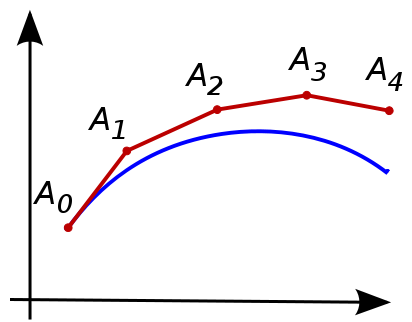
\includegraphics[width=0.7\linewidth]{figs/euler}
		\end{figure}
	\end{minipage}%
	\begin{minipage}[t]{0.6\columnwidth}
		\vspace{-0.2cm}
		\begin{figure}
			\centering
			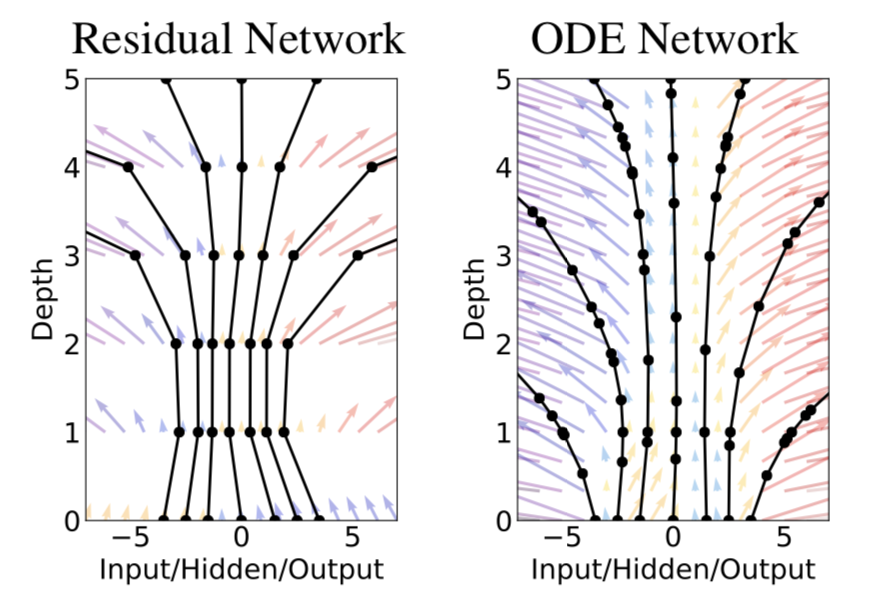
\includegraphics[width=0.9\linewidth]{figs/resnet_vs_neural_ode.png}
		\end{figure}
	\end{minipage}
	
	\myfootnotewithlink{https://arxiv.org/abs/1806.07366}{Chen R. T. Q. et al. Neural Ordinary Differential Equations, 2018}   
\end{frame}
%=======
\begin{frame}{Continuous-in-time Normalizing Flows}
	\vspace{-0.5cm}
	\begin{block}{Neural ODE}
		\vspace{-0.5cm}
		\begin{align*}
  \frac{d \bz(t)}{dt} &= \bff_{\btheta}(\bz(t), t); \quad \text{with initial condition }\bz(t_0) = \bz_0
		\end{align*}
		\vspace{-0.8cm}
	\end{block}
	\begin{minipage}[t]{0.6\columnwidth}
		\begin{itemize}
			\item Let $\bz(t_0)$ will be a random variable with some density function $p(\bz(t_0))$.
		 	\item Then $\bz(t_1)$ will be also a random variable with some other density function $p(\bz(t_1))$.
			\item We could say that we have the joint density function $p(\bz(t), t)$.
			\item What is the difference between $p(\bz(t), t)$ and $p(\bz, t)$?
		\end{itemize}
	\end{minipage}%
	\begin{minipage}[t]{0.4\columnwidth}	
		\begin{figure}
			\centering
			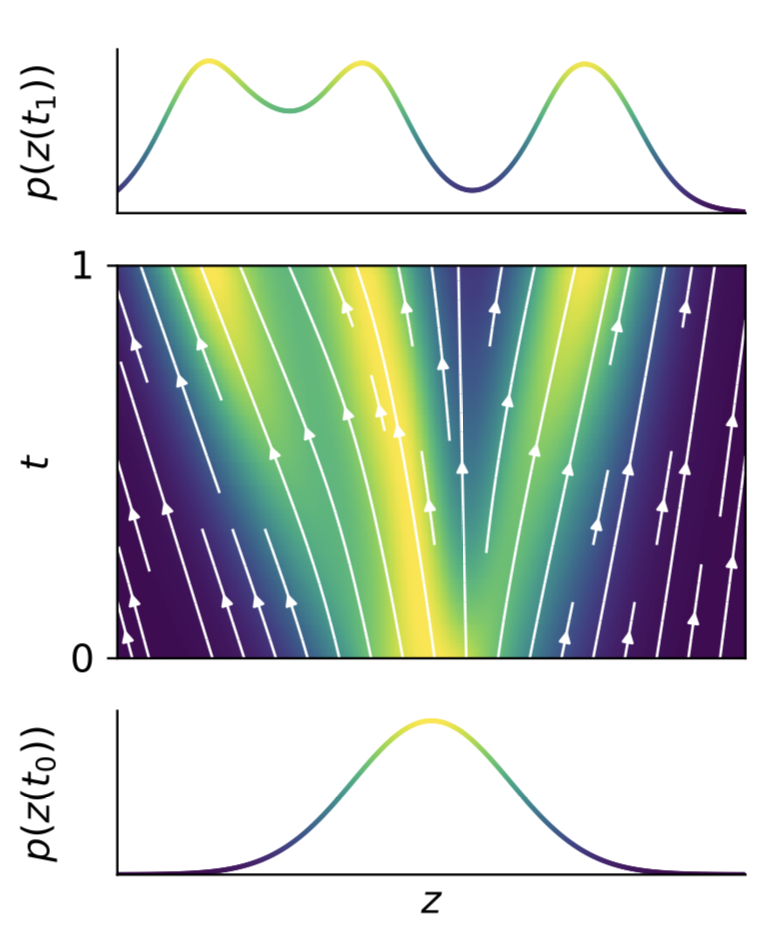
\includegraphics[width=\linewidth]{figs/cnf_flow.png}
		\end{figure}
	\end{minipage}
	\myfootnotewithlink{https://arxiv.org/abs/1810.01367}{Grathwohl W. et al. FFJORD: Free-form Continuous Dynamics for Scalable Reversible Generative Models, 2018}  
\end{frame}
%=======
\begin{frame}{Continuous-in-time Normalizing Flows}
	Let say that $p(\bz, t_0)$ is the base distribution (e.x. standard Normal) and $p(\bz, t_1)$ is the desired model distribution $p(\bx | \btheta)$.
	\begin{block}{Theorem (Picard)}
		If $\bff$ is uniformly Lipschitz continuous in $\bz$ and continuous in $t$, then the ODE has a \textbf{unique} solution.
	\end{block}
	It means that we are able \textbf{uniquely revert} our ODE. 
	\begin{block}{Forward and inverse transforms}
		\vspace{-0.7cm}
		\begin{align*}
			\bx &= \bz(t_1) = \bz(t_0) + \int_{t_0}^{t_1} \bff_{\btheta}(\bz(t), t) dt \\
			\bz &= \bz(t_0) = \bz(t_1) + \int_{t_1}^{t_0} \bff_{\btheta}(\bz(t), t) dt
		\end{align*}
		\vspace{-0.7cm}
	\end{block}
	\textbf{Note:} Unlike discrete-in-time NF, $\bff$ does not need to be bijective (uniqueness guarantees bijectivity).
	\myfootnotewithlink{https://arxiv.org/abs/1806.07366}{Chen R. T. Q. et al. Neural Ordinary Differential Equations, 2018}   
\end{frame}
%=======
\begin{frame}{Continuous-in-time Normalizing Flows}
	\begin{block}{What do we need?}
		\begin{itemize}
			\item We need the way to compute $p(\bz, t)$ at any moment $t$.
			\item We need the way to find the optimal parameters $\btheta$ of the dynamic $\bff_{\btheta}$.
		\end{itemize}
	\end{block}
	\vspace{-0.3cm}
	\begin{block}{Theorem (Kolmogorov-Fokker-Planck: special case)}
		If $\bff$ is uniformly Lipschitz continuous in $\bz$ and continuous in $t$, then
		\[
			\frac{d \log p(\bz(t), t)}{d t} = - \text{tr} \left( \frac{\partial \bff_{\btheta}(\bz(t), t)}{\partial \bz(t)} \right).
		\]
		\[
			\log p(\bz(t_1), t_1) = \log p(\bz(t_0), t_0) - \int_{t_0}^{t_1} \text{tr}  \left( \frac{\partial \bff_{\btheta}(\bz(t), t)}{\partial \bz(t)} \right) dt.
		\]
	\end{block}
	It means that if we have the value $\bz_0 = \bz(t_0)$ then the solution of the ODE will give us the density at the moment $t_1$.
	\myfootnotewithlink{https://arxiv.org/abs/1806.07366}{Chen R. T. Q. et al. Neural Ordinary Differential Equations, 2018}   
\end{frame}
%=======
\begin{frame}{Continuous-in-time Normalizing Flows}
	\begin{block}{Forward transform + log-density}
		\vspace{-0.7cm}
		\begin{align*}
				\bx &= \bz + \int_{t_0}^{t_1} \bff_{\btheta}(\bz(t), t) dt \\
				\log p(\bx | \btheta) &= \log p(\bz) - \int_{t_0}^{t_1} \text{tr} \left( \frac{\partial \bff_{\btheta}(\bz(t), t)}{\partial \bz(t)} \right) dt
		\end{align*}
		Here $p(\bx | \btheta) = p(\bz(t_1), t_1)$, $p(\bz) = p(\bz(t_0), t_0)$.
	\end{block}
	\begin{itemize}
		\item \textbf{Discrete-in-time NF}: evaluation of determinant of the Jacobian costs $O(m^3)$ (we need invertible $\bff$).
		\item \textbf{Continuous-in-time NF}: getting the trace of the Jacobian costs $O(m^2)$ (we need smooth $\bff$).
	\end{itemize}
	\begin{block}{Why $O(m^2)$?}
		$\text{tr} \left( \frac{\partial \bff_{\btheta}(\bz(t))}{\partial \bz(t)} \right)$ costs $O(m^2)$ ($m$ evaluations of $\bff$), since we have to compute a derivative for each diagonal element. It is possible to reduce cost from $O(m^2)$ to $O(m)$!
	\end{block}
	\myfootnotewithlink{https://arxiv.org/abs/1806.07366}{Chen R. T. Q. et al. Neural Ordinary Differential Equations, 2018}   
\end{frame}
%=======
\begin{frame}{Continuous-in-time Normalizing Flows}
	\begin{block}{Hutchinson's trace estimator}
		If $\bepsilon \in \bbR^m$ is a random variable with $\mathbb{E} [\bepsilon] = 0$ and $\text{cov} (\bepsilon) = \bI$, then
		\vspace{-0.3cm}
		\begin{multline*}
		    \text{tr}(\mathbf{A}) = \text{tr}\left(\mathbf{A} \cdot {\color{olive}\bI} \right) = \text{tr}\left(\mathbf{A} \cdot {\color{olive}\mathbb{E}_{p(\bepsilon)} \left[ \bepsilon \bepsilon^T \right]} \right) = \\ 
		    =  \mathbb{E}_{p(\bepsilon)} \left[  \text{tr}\left(  \mathbf{A}  \bepsilon \bepsilon^T \right) \right] =  \mathbb{E}_{p(\bepsilon)} \left[ {\color{violet} \bepsilon^T \mathbf{A}} \bepsilon  \right]
		\end{multline*}
		\vspace{-0.6 cm}
	\end{block}
	Jacobian vector products ${\color{violet}\bv^T \frac{\partial f}{\partial \bz}}$ can be computed for approximately the same cost as evaluating $\bff$ (\texttt{torch.autograd.functional.jvp}).
	\begin{block}{FFJORD density estimation}
		\vspace{-0.8cm}
		\begin{multline*}
		    \log p(\bz(t_1)) = \log p(\bz(t_0)) - \int_{t_0}^{t_1} \text{tr}  \left( \frac{\partial \bff_{\btheta}(\bz(t), t)}{\partial \bz(t)} \right) dt = \\ = \log p(\bz(t_0)) - \mathbb{E}_{p(\bepsilon)} \int_{t_0}^{t_1} \left[ {\color{violet}\bepsilon^T \frac{\partial \bff}{\partial \bz}} \bepsilon \right] dt.
		\end{multline*}
	\end{block}
	\myfootnotewithlink{https://arxiv.org/abs/1810.01367}{Grathwohl W. et al. FFJORD: Free-form Continuous Dynamics for Scalable Reversible Generative Models, 2018} 
\end{frame}
%=======
\section{Continuous-in-time NF: adjoint method}
%=======
\begin{frame}{Neural ODE}
	\begin{block}{Continuous-in-time NF}
		{\small
		\begin{minipage}[t]{0.4\columnwidth}
			\[
	 			 \frac{d \bz(t)}{dt} = \bff_{\btheta}(\bz(t), t) 	 
	 		\]
	 		\[
	 			 \bx = \bz + \int_{t_0}^{t_1} \bff_{\btheta}(\bz(t), t) dt 
			\]
		\end{minipage}% 
		\begin{minipage}[t]{0.6\columnwidth}
			\vspace{-0.4cm}
			\[
					\frac{d \log p(\bz(t), t)}{d t} = - \text{tr} \left( \frac{\partial \bff_{\btheta}(\bz(t), t)}{\partial \bz(t)} \right) 
	 		\]
	 		\[
					\log p(\bx | \btheta) = \log p(\bz) - \int_{t_0}^{t_1} \text{tr} \left( \frac{\partial \bff_{\btheta}(\bz(t), t)}{\partial \bz(t)} \right) dt
			\]
		\end{minipage}
		}
	\end{block}
	How to get optimal parameters of $\btheta$? \\
	
	For fitting parameters we need gradients. We need the analogue of the backpropagation.
	\begin{block}{Forward pass (Loss function)}
		\vspace{-0.3cm}
		\[
			\bz = \bx + \int_{t_1}^{t_0} \bff_{\btheta}(\bz(t), t) dt, \quad L(\bz) = - \log p(\bx | \btheta)
		\]
		\[
			L(\bz) = - \log p(\bz) + \int_{t_0}^{t_1} \text{tr} \left( \frac{\partial \bff_{\btheta}(\bz(t), t)}{\partial \bz(t)} \right) dt
		\]
	\end{block}
	\myfootnotewithlink{https://arxiv.org/abs/1806.07366}{Chen R. T. Q. et al. Neural Ordinary Differential Equations, 2018}     
\end{frame}
%=======
\begin{frame}{Neural ODE}
	\vspace{-0.2cm}
	\begin{block}{Adjoint functions}
		\vspace{-0.4cm}
		\[
			\ba_{\bz}(t) = \frac{\partial L}{\partial \bz(t)}; \quad \ba_{\btheta}(t) = \frac{\partial L}{\partial \btheta(t)}.
		\]
		These functions show how the gradient of the loss depends on the hidden state~$\bz(t)$ and parameters $\btheta$.
		\vspace{-0.3cm}
	\end{block}

	\begin{block}{Theorem (Pontryagin)}
		\vspace{-0.6cm}
		\[
		\frac{d \ba_{\bz}(t)}{dt} = - \ba_{\bz}(t)^T \cdot \frac{\partial \bff_{\btheta}(\bz(t), t)}{\partial \bz}; \quad \frac{d \ba_{\btheta}(t)}{dt} = - \ba_{\bz}(t)^T \cdot \frac{\partial \bff_{\btheta}(\bz(t),  t)}{\partial \btheta}.
		\]
		\vspace{-0.7cm}
	\end{block}
	\begin{block}{Solution for adjoint function}
		\vspace{-0.6cm}
		{\small
		\begin{align*}
			\frac{\partial L}{\partial \btheta(t_1)} &= \ba_{\btheta}(t_1) =  - \int_{t_0}^{t_1} \ba_{\bz}(t)^T \frac{\partial \bff_{\btheta}(\bz(t), t)}{\partial \btheta(t)} dt + 0\\
			\frac{\partial L}{\partial \bz(t_1)} &= \ba_{\bz}(t_1) =  - \int_{t_0}^{t_1} \ba_{\bz}(t)^T \frac{\partial \bff_{\btheta}(\bz(t), t)}{\partial \bz(t)} dt + \frac{\partial L}{\partial \bz(t_0)}\\
		\end{align*}
		}
		\vspace{-1.3cm}
	\end{block}
	\textbf{Note:} These equations are solved in reverse time direction.
	\myfootnotewithlink{https://arxiv.org/abs/1806.07366}{Chen R. T. Q. et al. Neural Ordinary Differential Equations, 2018}   
\end{frame}
%=======
\begin{frame}{Adjoint method}
	\begin{block}{Forward pass}
		\vspace{-0.3cm}
		\[
		\bz = \bz(t_0) = \int^{t_1}_{t_0} \bff_{\btheta}(\bz(t), t) d t  + \bx \quad \Rightarrow \quad \text{ODE Solver}
		\]
		\vspace{-0.4cm}
	\end{block}
	\begin{block}{Backward pass}
		\vspace{-0.5cm}
		\begin{equation*}
			\left.
			{\footnotesize 
				\begin{aligned}
					\frac{\partial L}{\partial \btheta(t_1)} &= \ba_{\btheta}(t_1) =  - \int_{t_0}^{t_1} \ba_{\bz}(t)^T \frac{\partial \bff_{\btheta}(\bz(t), t)}{\partial \btheta(t)} dt + 0 \\
					\frac{\partial L}{\partial \bz(t_1)} &= \ba_{\bz}(t_1) =  - \int_{t_0}^{t_1} \ba_{\bz}(t)^T \frac{\partial \bff_{\btheta}(\bz(t), t)}{\partial \bz(t)} dt + \frac{\partial L}{\partial \bz(t_0)} \\
					\bz(t_1) &= - \int^{t_0}_{t_1} \bff_{\btheta}(\bz(t), t) d t  + \bz_0.
				\end{aligned}
			}
			\right\rbrace
			\Rightarrow
			\text{ODE Solver}
		\end{equation*}
		\vspace{-0.4cm} 
	\end{block}
	\textbf{Note:} These scary formulas are the standard backprop in the discrete case.
	\myfootnotewithlink{https://arxiv.org/abs/1806.07366}{Chen R. T. Q. et al. Neural Ordinary Differential Equations, 2018}   
\end{frame}
%=======
\section{SDE basics}
%=======
\begin{frame}{Ordinary differential equation (ODE)}
	\begin{block}{Continuous-in-time Normalizing Flows}
		\vspace{-0.3cm}
		\[
  			\frac{d \bz(t)}{dt} = \bff_{\btheta}(\bz(t), t); \quad \text{with initial condition }\bz(t_0) = \bz_0
		\]
		\vspace{-0.5cm}
	\end{block}
	\begin{minipage}[t]{0.6\columnwidth}
		\begin{itemize}
			\item Let $\bz(t_0)$ will be a random variable with some density function $p(\bz(t_0))$.
		 	\item Then $\bz(t_1)$ will be also a random variable with some other density function $p(\bz(t_1))$.
			\item We could say that we have the joint density function $p(\bz(t), t)$.
			\item What is the difference between $p(\bz(t), t)$ and $p(\bz, t)$?
		\end{itemize}
	\end{minipage}%
	\begin{minipage}[t]{0.4\columnwidth}	
		\begin{figure}
			\centering
			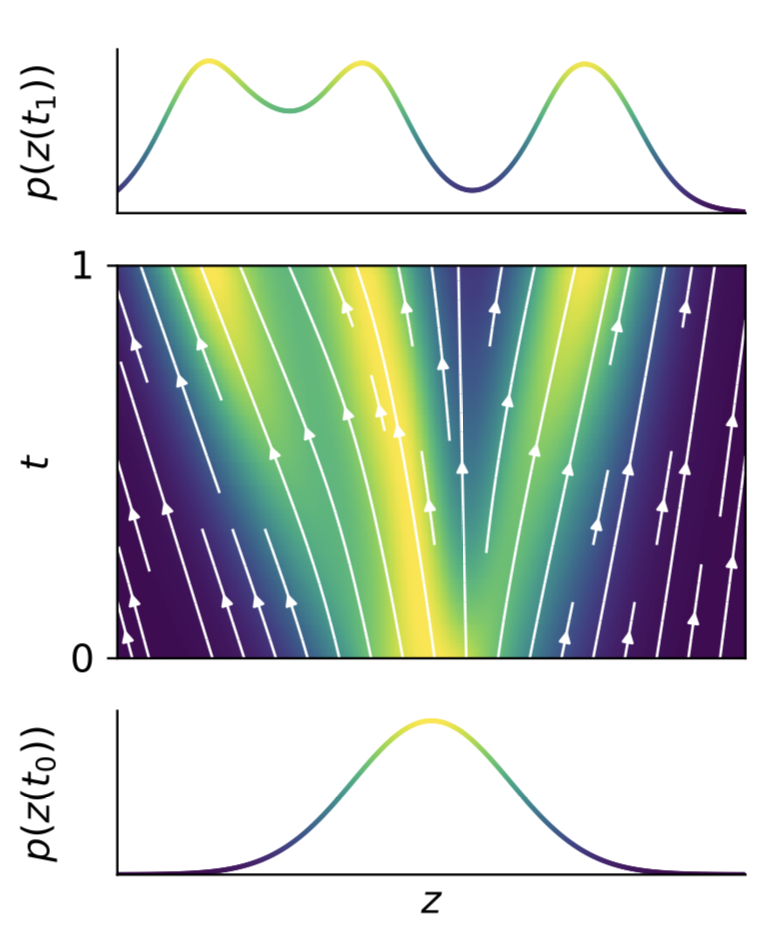
\includegraphics[width=\linewidth]{figs/cnf_flow.png}
		\end{figure}
	\end{minipage}
	\myfootnotewithlink{https://arxiv.org/abs/1810.01367}{Grathwohl W. et al. FFJORD: Free-form Continuous Dynamics for Scalable Reversible Generative Models, 2018}  
\end{frame}
%=======
\begin{frame}{Ordinary differential equation (ODE)}
	\[
 			d \bz = \bff_{\btheta}(\bz, t) \cdot dt
	\]
	\vspace{-0.5cm}
	\begin{block}{Discretization of ODE (Euler method)}
		\vspace{-0.3cm}
		\[
			\bz(t + dt) = \bz(t) + \bff_{\btheta}(\bz(t), t) \cdot dt
		\]
		\vspace{-0.5cm}
	\end{block}
	\begin{block}{Theorem (Kolmogorov-Fokker-Planck: special case)}
		If $\bff$ is uniformly Lipschitz continuous in $\bz$ and continuous in $t$, then
		\[
			\frac{d \log p(\bz(t), t)}{d t} = - \text{tr} \left( \frac{\partial \bff_{\btheta}(\bz(t), t)}{\partial \bz(t)} \right).
		\]
	\end{block}
	It means that if we have the value $\bz_0 = \bz(t_0)$ then the solution of the ODE will give us the density at the moment $t_1$.
	\myfootnotewithlink{https://arxiv.org/abs/1806.07366}{Chen R. T. Q. et al. Neural Ordinary Differential Equations, 2018}   
\end{frame}
%=======
\begin{frame}{Stochastic differential equation (SDE)}
	Let define stochastic process $\bx(t)$ with initial condition $\bx(0) \sim p_0(\bx) = \pi(\bx)$:
	\[
		d\bx = \mathbf{f}(\bx, t) dt + g(t) d \bw
	\]
	\vspace{-0.5cm}
	\begin{itemize}
		 \item $\mathbf{f}(\bx, t): \bbR^m \times [0, 1] \rightarrow \bbR^m$ is the \textbf{drift} function of $\bx(t)$.
		 \item $g(t): \bbR \rightarrow \bbR$ is the \textbf{diffusion} function of $\bx(t)$.
		 \item $\bw(t)$ is the standard Wiener process (Brownian motion):
		 \begin{enumerate}
		 	\item $\bw(0) = 0$ (almost surely);
		 	\item $\bw(t)$ has independent increments;
			 \item $\bw(t) - \bw(s) \sim \cN(0, (t - s) \bI)$, for $t > s$.
		 \end{enumerate}
		 \item $d \bw = \bw(t + dt) - \bw(t) = \cN(0, \bI \cdot dt ) = \bepsilon \cdot \sqrt{dt}$, where $\bepsilon \sim \cN(0, \bI)$.
		 \item If $g(t) = 0$ we get standard ODE.
	\end{itemize}
\end{frame}
%=======
\begin{frame}{Stochastic differential equation (SDE)}
	\[
		d\bx = \mathbf{f}(\bx, t) dt + g(t) d \bw
	\]
	\vspace{-0.3cm}
	\begin{itemize}
		\item In contrast to ODE, initial condition $\bx(0)$ does not uniquely determine the process trajectory.
		\item We have two sources of randomness: initial distribution $p_0(\bx)$ and Wiener process $\bw(t)$.
	\end{itemize}
	\begin{block}{Discretization of SDE (Euler method)}
		\vspace{-0.3cm}
		\[
			\bx(t + dt) = \bx(t) + \bff(\bx(t), t) \cdot dt + g(t) \cdot \bepsilon \cdot \sqrt{dt}
		\]
		If $dt = 1$, then
		\vspace{-0.3cm}
		\[
			\bx_{t + 1} = \bx_t + \bff(\bx_t, t) + g(t) \cdot \bepsilon
		\]
		\vspace{-0.7cm}
	\end{block}
	\begin{itemize}
		\item At each moment $t$ we have the density $p(\bx(t), t)$.
		\item $p: \bbR^m \times [0, 1] \rightarrow \bbR_+$ is a \textbf{probability path} between $p_0(\bx)$ and $p_1(\bx)$.
		\item How to get the distribution path $p(\bx, t)$ for $\bx(t)$?
	\end{itemize}
\end{frame}
%=======
\begin{frame}{Stochastic differential equation (SDE)}
	\vspace{-0.4cm}
	\[
		d\bx = \mathbf{f}(\bx, t) dt + g(t) d \bw, \quad d \bw = \bepsilon \cdot \sqrt{dt}, \quad \bepsilon \sim \cN(0, \bI).
	\]
	\vspace{-0.4cm}
 	\begin{block}{Theorem (Kolmogorov-Fokker-Planck)}
 		Evolution of the distribution $p(\bx, t)$ is given by the following equation:
 		\vspace{-0.2cm}
 		\[
 			\frac{\partial p(\bx, t)}{\partial t} = - \text{div}\left(\bff(\bx, t) p(\bx, t)\right) + \frac{1}{2}g^2(t) \Delta_{\bx}p(\bx, t)
 		\]
 		Here
 		\[
 			\text{div} (\bv) = \sum_{i=1}^m \frac{\partial v_i(\bx)}{\partial x_i} = \text{tr}\left( \frac{\partial \bv(\bx)}{\partial \bx}  \right)
 		\]
 		\[
 			\Delta_{\bx}p(\bx, t) = \sum_{i=1}^m \frac{\partial^2 p(\bx, t)}{\partial x_i^2} = \text{tr}\left( \frac{\partial^2 p(\bx, t)}{\partial \bx^2}  \right)
 		\]
 		\[
 			\frac{\partial p(\bx, t)}{\partial t} = \text{tr}\left(- \frac{\partial}{\partial \bx} \bigl[ \mathbf{f}(\bx, t) p(\bx, t)\bigr] + \frac{1}{2} g^2(t) \frac{\partial^2 p(\bx, t)}{\partial \bx^2} \right)
 		\]
 	\end{block}
\end{frame}
%=======
\begin{frame}{Stochastic differential equation (SDE)}
 	\begin{block}{Theorem (Kolmogorov-Fokker-Planck)}
 		\vspace{-0.2cm}
 		\[
 			\frac{\partial p(\bx, t)}{\partial t} = \text{tr}\left(- \frac{\partial}{\partial \bx} \bigl[ \mathbf{f}(\bx, t) p(\bx, t)\bigr] + \frac{1}{2} g^2(t) \frac{\partial^2 p(\bx, t)}{\partial \bx^2} \right)
 		\]
 	\end{block}
 	 \begin{itemize}
 	 	\item KFP theorem uniquely defines the SDE.
 		 \item This is the generalization of KFP theorem that we used in continuous-in-time NF:
 	 	\[
 	 		\frac{d \log p(\bx(t), t)}{d t} = - \text{tr} \left( \frac{\partial \bff(\bx, t)}{\partial \bx} \right).
 	 	\]
 	 \end{itemize}
	\vspace{-0.3cm}
 	\begin{block}{Langevin SDE (special case)}
 		\vspace{-0.6cm}
 		\begin{align*}
 			d\bx &= {\color{violet}\mathbf{f}(\bx, t)} dt + {\color{teal}g(t)} d \bw \\
 			d \bx &= {\color{violet}\frac{1}{2} \frac{\partial}{\partial \bx} \log p(\bx, t)} d t + {\color{teal} 1 } \cdot d \bw
 		\end{align*}
 		\vspace{-0.3cm}
 	\end{block}
 	Let apply KFP theorem to this SDE.
\end{frame}
%=======
\begin{frame}{Langevin SDE (special case)}
	\[
		d \bx = \frac{1}{2} \frac{\partial}{\partial \bx} \log p(\bx, t) d t + 1 \cdot d \bw
	\]
	\begin{multline*}
		\frac{\partial p(\bx, t)}{\partial t} =  \text{tr} \left(- \frac{\partial}{\partial \bx}\left[ {\color{olive}p(\bx, t) \frac{1}{2} \frac{\partial}{\partial \bx} \log p(\bx, t)} \right]  + \frac{1}{2} \frac{\partial^2 p(\bx, t)}{\partial \bx^2} \right) = \\
		= \text{tr} \left(- \frac{\partial}{\partial \bx}\left[ {\color{olive}\frac{1}{2} \frac{\partial}{\partial \bx} p(\bx, t) } \right]  + \frac{1}{2} \frac{\partial^2 p(\bx, t)}{\partial \bx^2} \right) = 0
	\end{multline*}
	The density $p(\bx, t) = \text{const}(t)$! \\ If $\bx(0) \sim p_0(\bx)$, then $\bx(t) \sim p_0(\bx)$.
	\begin{block}{Discretized Langevin SDE}
		\vspace{-0.3cm}
		\[
			\bx_{t + 1} - \bx_t = \frac{\eta}{2} \cdot \frac{\partial}{\partial \bx} \log p(\bx, t) + \sqrt{\eta} \cdot \bepsilon, \quad \eta \approx dt.
		\]
		\vspace{-0.4cm}
	\end{block}
	\begin{block}{Langevin dynamic}
		\vspace{-0.3cm}
		\[
			\bx_{t + 1} = \bx_t + \frac{\eta}{2} \cdot \nabla_{\bx} \log p(\bx | \btheta) + \sqrt{\eta} \cdot \bepsilon, \quad \eta \approx dt.
		\]
		\vspace{-0.3cm}
	\end{block}
\end{frame}
%=======
\section{Probability flow ODE}
%=======
\begin{frame}{Probability flow ODE}
	\begin{block}{Theorem}
		Assume SDE $d\bx = \mathbf{f}(\bx, t) dt + g(t) d \bw$ induces the probability path $p(\bx, t)$.
		Then there exists ODE with identical probability path $p(\bx, t)$ of the form
		\vspace{-0.3cm}
		\[
			d\bx = \left[\mathbf{f}(\bx, t) -\frac{1}{2} g^2(t) \frac{\partial}{\partial \bx} \log p(\bx, t) \right] dt
		\]
		\vspace{-0.7cm}
	\end{block}
	\begin{block}{Proof}
 		\vspace{-0.7cm}
 		{\small
 		\begin{multline*}
 			\frac{\partial p(\bx, t)}{\partial t} = \text{tr}\left(- \frac{\partial}{\partial \bx} \bigl[ \mathbf{f}(\bx, t) p(\bx, t)\bigr] + \frac{1}{2} g^2(t) \frac{\partial^2 p(\bx, t)}{\partial \bx^2} \right) = \\
 			=  \text{tr}\left(- \frac{\partial}{\partial \bx} \left[ \mathbf{f}(\bx, t) p(\bx, t) - \frac{1}{2} g^2(t) {\color{violet}\frac{\partial p(\bx, t)}{\partial \bx}} \right]  \right) = \\
			 =  \text{tr}\left(- \frac{\partial}{\partial \bx} \left[ \mathbf{f}(\bx, t) p(\bx, t) - \frac{1}{2} g^2(t) {\color{violet}p(\bx, t) \frac{\partial \log p(\bx, t)}{\partial \bx}} \right]  \right)= \\
		  =  \text{tr}\left(- \frac{\partial}{\partial \bx} \left[ \left( {\color{teal}\mathbf{f}(\bx, t) - \frac{1}{2} g^2(t) \frac{\partial \log p(\bx, t)}{\partial \bx}}\right) p(\bx, t) \right]  \right)
 		\end{multline*}
 		}
 	\end{block}
	\myfootnotewithlink{https://arxiv.org/abs/2011.13456}{Song Y., et al. Score-Based Generative Modeling through Stochastic Differential Equations, 2020}
\end{frame}
\begin{frame}{Probability flow ODE}
	\begin{block}{Theorem}
		Assume SDE $d\bx = \mathbf{f}(\bx, t) dt + g(t) d \bw$ induces the distribution $p(\bx, t)$.
		Then there exists ODE with identical probabilities distribution $p(\bx, t)$ of the form
		\vspace{-0.3cm}
		\[
			d\bx = \left[\mathbf{f}(\bx, t) -\frac{1}{2} g^2(t) \frac{\partial}{\partial \bx} \log p(\bx, t) \right] dt
		\]
		\vspace{-0.7cm}
	\end{block}
	\begin{block}{Proof (continued)}
 		\vspace{-0.7cm}
 		\begin{multline*}
 			\frac{\partial p(\bx, t)}{\partial t} =  \text{tr}\left(- \frac{\partial}{\partial \bx} \left[ \left( {\color{teal}\mathbf{f}(\bx, t) - \frac{1}{2} g^2(t) \frac{\partial \log p(\bx, t)}{\partial \bx}}\right) p(\bx, t) \right]  \right) =\\
 			  =  \text{tr}\left(- \frac{\partial}{\partial \bx} \left[ {\color{teal}\tilde{\mathbf{f}}(\bx, t)} p(\bx, t) \right]  \right)
 		\end{multline*}
 	\end{block}
 	\vspace{-1.0cm}
 	\[
 		d \bx = \tilde{\bff}(\bx, t) dt + 0 \cdot d \bw = \left[\mathbf{f}(\bx, t) -\frac{1}{2} g^2(t) \frac{\partial}{\partial \bx} \log p(\bx, t) \right] dt
 	\]
	\myfootnotewithlink{https://arxiv.org/abs/2011.13456}{Song Y., et al. Score-Based Generative Modeling through Stochastic Differential Equations, 2020}
\end{frame}
%=======
\begin{frame}{Probability flow ODE}
	\vspace{-0.5cm}
	\begin{align*}
		d\bx &= \mathbf{f}(\bx, t) dt + g(t) d \bw - \text{SDE} \\
		d\bx &= \left[\mathbf{f}(\bx, t) -\frac{1}{2} g^2(t) \frac{\partial}{\partial \bx} \log p(\bx, t) \right] dt  - \text{probability flow ODE}
	\end{align*}
	\vspace{-0.3cm}
	\begin{itemize}
		\item The term $\bs(\bx, t) = \frac{\partial}{\partial \bx} \log p(\bx, t)$ is a score function for continuous time.
		\item ODE has more stable trajectories.
	\end{itemize}
	\begin{figure}
		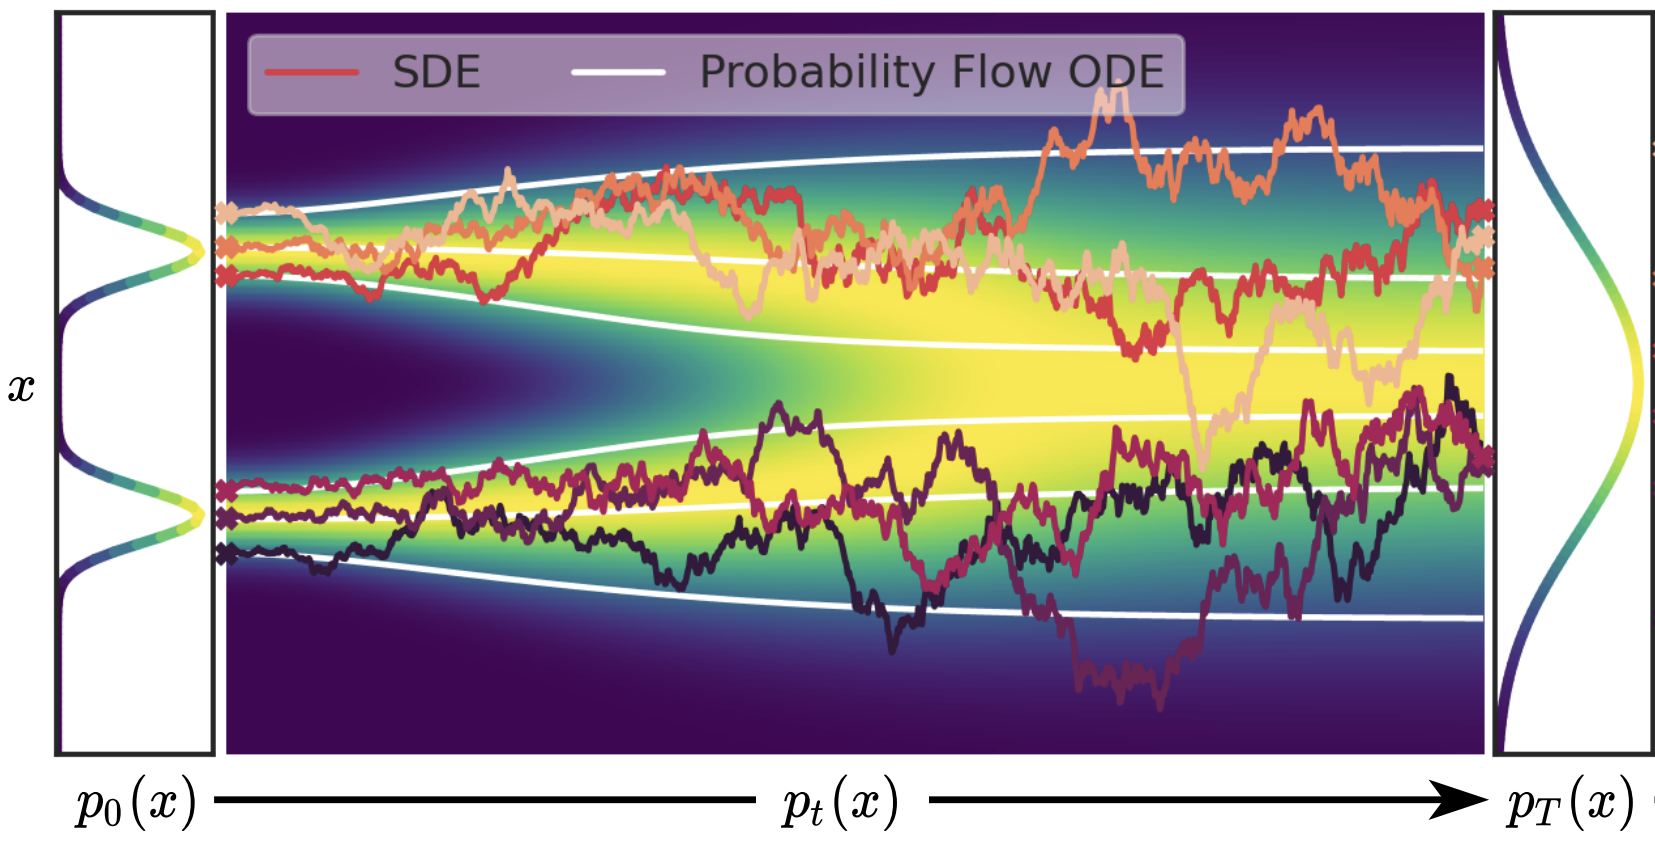
\includegraphics[width=0.75\linewidth]{figs/probability_flow}
	\end{figure}
	\myfootnotewithlink{https://arxiv.org/abs/2011.13456}{Song Y., et al. Score-Based Generative Modeling through Stochastic Differential Equations, 2020}
\end{frame}
%=======
\section{Reverse SDE}
%=======
\begin{frame}{Reverse SDE}
	\vspace{-0.3cm}
	\[
		d\bx = \mathbf{f}(\bx, t) dt, \quad \bx(t + dt) = \bx(t) + \mathbf{f}(\bx, t) dt
	\]
	Here $dt$ could be $>0$ or $<0$. 
	\begin{block}{Reverse ODE}
		Let $\tau = 1 - t$ ($d\tau = -dt$).
		\vspace{-0.3cm}
		\[
			d\bx = - \bff(\bx, 1 - \tau) d \tau
		\]
	\end{block}
	\vspace{-0.5cm}
	\begin{itemize}
		\item How to revert SDE $d\bx = \mathbf{f}(\bx, t) dt + g(t) d \bw$? 
		\item Wiener process gives the randomness that we have to revert.
	\end{itemize}
	\vspace{-0.3cm}
	\begin{block}{Theorem}
		There exists the reverse SDE for the SDE $d\bx = \mathbf{f}(\bx, t) dt + g(t) d \bw$ that has the following form
		\vspace{-0.3cm}
		\[
			d\bx = \left(\mathbf{f}(\bx, t) {\color{violet}- g^2(t) \frac{\partial \log p(\bx, t)}{\partial \bx}}\right) dt + g(t) d \bw
		\]
		\vspace{-0.5cm} \\
		with $dt < 0$.
	\end{block}
	\myfootnotewithlink{https://arxiv.org/abs/2011.13456}{Song Y., et al. Score-Based Generative Modeling through Stochastic Differential Equations, 2020}
\end{frame}
%=======
\begin{frame}{Reverse SDE}
	\begin{block}{Theorem}
		There exists the reverse SDE for the SDE $d\bx = \mathbf{f}(\bx, t) dt + g(t) d \bw$ that has the following form
		\vspace{-0.3cm}
		\[
			d\bx = \left(\mathbf{f}(\bx, t) {\color{violet}- g^2(t) \frac{\partial \log p(\bx, t)}{\partial \bx}}\right) dt + g(t) d \bw
		\]
		\vspace{-0.5cm} \\
		with $dt < 0$.
	\end{block}
	\textbf{Note:} Here we also see the score function $\bs(\bx, t) = \frac{\partial}{\partial \bx} \log p(\bx, t)$.
	\begin{block}{Sketch of the proof}
		\begin{itemize}
			\item Convert initial SDE to probability flow ODE.
			\item Revert probability flow ODE.
			\item Convert reverse probability flow ODE to reverse SDE.
		\end{itemize}
	\end{block}
	\myfootnotewithlink{https://arxiv.org/abs/2011.13456}{Song Y., et al. Score-Based Generative Modeling through Stochastic Differential Equations, 2020}
\end{frame}
%=======
\begin{frame}{Reverse SDE}
	\begin{block}{Proof}
		\begin{itemize}
			\item Convert initial SDE to probability flow ODE
			\vspace{-0.1cm}
			{\footnotesize
			\begin{align*}
				d\bx &= \mathbf{f}(\bx, t) dt + g(t) d \bw \\
				d\bx &= \left[\mathbf{f}(\bx, t) -\frac{1}{2} g^2(t) \frac{\partial}{\partial \bx} \log p(\bx, t) \right] dt
			\end{align*}
			}
			\item Revert probability flow ODE
			\vspace{-0.1cm}
			{\footnotesize
			\begin{align*}
				d\bx &= \left[\mathbf{f}(\bx, t) -\frac{1}{2} g^2(t) \frac{\partial}{\partial \bx} \log p(\bx, t) \right] dt \\
				d\bx &= \left[- \mathbf{f}(\bx, 1 - \tau) + \frac{1}{2} g^2(1 - \tau) \frac{\partial}{\partial \bx} \log p(\bx, 1 - \tau) \right] d \tau
			\end{align*}
			}
			\item Convert reverse probability flow ODE to reverse SDE
			\vspace{-0.1cm}
			{\footnotesize
			\begin{align*}
				d\bx &= \left[- \mathbf{f}(\bx, 1 - \tau) + \frac{1}{2} g^2(1 - \tau) \frac{\partial}{\partial \bx} \log p(\bx, 1 - \tau) \right] d \tau \\
				d\bx &= \left[- \mathbf{f}(\bx, 1 - \tau) + g^2(1 - \tau) \frac{\partial}{\partial \bx} \log p(\bx, 1 - \tau) \right] d\tau + g(1 - \tau) d \bw
			\end{align*}
			}
		\end{itemize}
	\end{block}
	\myfootnotewithlink{https://arxiv.org/abs/2011.13456}{Song Y., et al. Score-Based Generative Modeling through Stochastic Differential Equations, 2020}
\end{frame}
%=======
\begin{frame}{Reverse SDE}
	\begin{block}{Theorem}
		There exists the reverse SDE for the SDE $d\bx = \mathbf{f}(\bx, t) dt + g(t) d \bw$ that has the following form
		\vspace{-0.3cm}
		\[
			d\bx = \left(\mathbf{f}(\bx, t) {\color{violet}- g^2(t) \frac{\partial \log p(\bx, t)}{\partial \bx}}\right) dt + g(t) d \bw
		\]
		\vspace{-0.5cm} \\
		with $dt < 0$.
	\end{block}
	\begin{block}{Proof (continued)}
		\vspace{-0.7cm}
		\[
			d\bx = \left[- \mathbf{f}(\bx, 1 - \tau) + g^2(1 - \tau) \frac{\partial}{\partial \bx} \log p(\bx, 1 - \tau) \right] d \tau + g(1 - \tau) d \bw
		\]
		\[
			d\bx = \left(\mathbf{f}(\bx, t) - g^2(t) \frac{\partial \log p(\bx, t)}{\partial \bx}\right) dt + g(t) d \bw
		\]
		Here $d\tau > 0$ and $dt < 0$.
	\end{block}
	\myfootnotewithlink{https://arxiv.org/abs/2011.13456}{Song Y., et al. Score-Based Generative Modeling through Stochastic Differential Equations, 2020}
\end{frame}
%=======
\begin{frame}{Reverse SDE}
	\vspace{-0.5cm}
	\begin{align*}
		d\bx &= \mathbf{f}(\bx, t) dt + g(t) d \bw - \text{SDE} \\
		d\bx &= \left[\mathbf{f}(\bx, t) -\frac{1}{2} g^2(t) \frac{\partial}{\partial \bx} \log p(\bx, t) \right] dt - \text{probability flow ODE} \\
		d\bx &= \left(\mathbf{f}(\bx, t) - g^2(t) \frac{\partial \log p(\bx, t)}{\partial \bx}\right) dt + g(t) d \bw - \text{reverse SDE}
	\end{align*}
	\vspace{-0.5cm}
	\begin{itemize}
		\item We got the way to transform one distribution to another via SDE with some probability path $p(\bx, t)$.
		\item We are able to revert this process with the score function.
	\end{itemize}
	\vspace{-0.3cm}
	\begin{figure}
		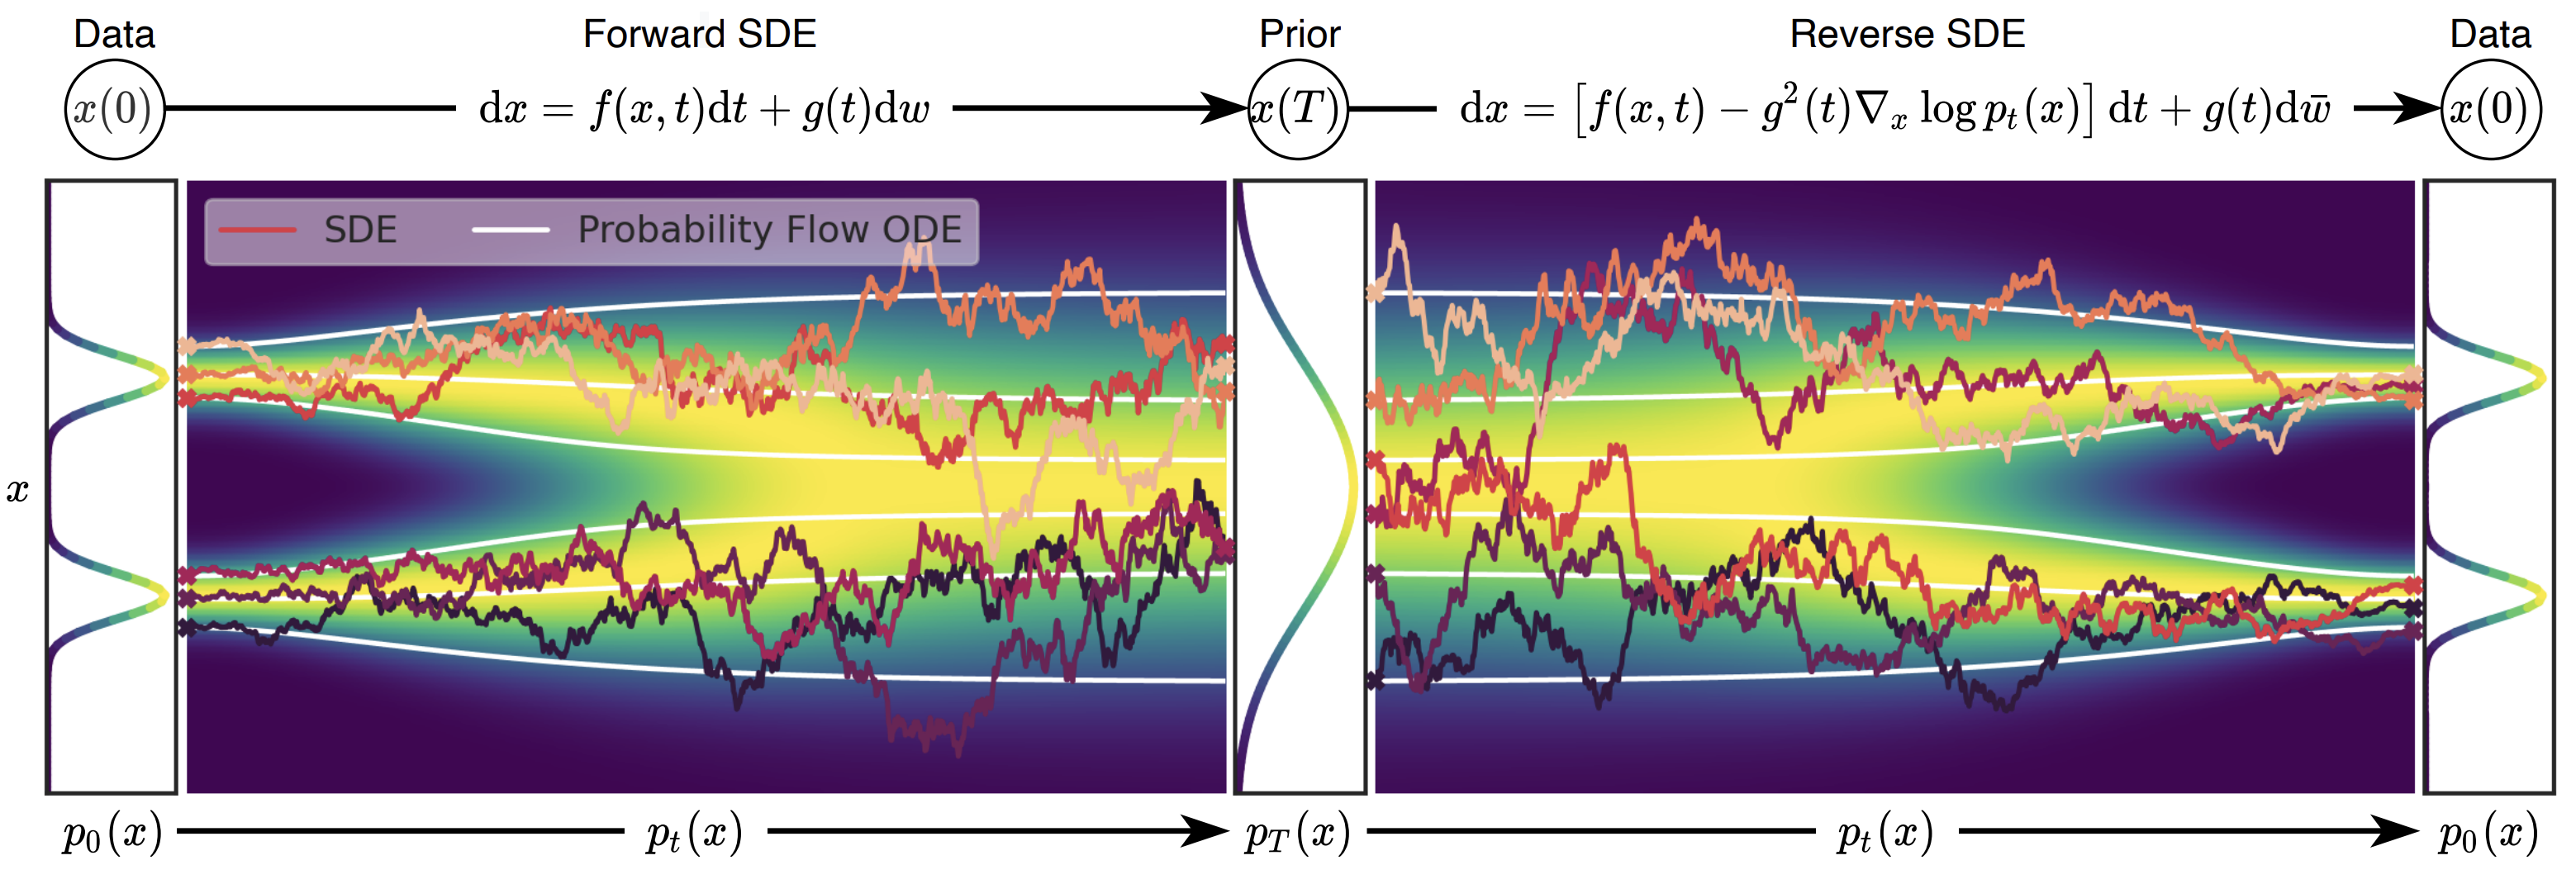
\includegraphics[width=0.9\linewidth]{figs/sde}
	\end{figure}
	\myfootnotewithlink{https://arxiv.org/abs/2011.13456}{Song Y., et al. Score-Based Generative Modeling through Stochastic Differential Equations, 2020}
\end{frame}
%=======
\section{Diffusion and Score matching SDEs}
%=======
\begin{frame}{Score matching SDE}
	\begin{block}{Denoising score matching}
		\vspace{-0.7cm}
		\begin{align*}
			\bx_t &= \bx + \sigma_t \cdot \bepsilon_t, \quad p(\bx, \sigma_t) = \cN(\bx, \sigma_t^2 \cdot \bI) \\
			\bx_{t-1} &= \bx + \sigma_{t-1} \cdot \bepsilon_{t-1}, \quad p(\bx, \sigma_{t-1}) = \cN(\bx, \sigma_{t-1}^2 \cdot \bI)
		\end{align*}
	\end{block}
	\vspace{-1.0cm}
	\[
		\bx_t = \bx_{t - 1} + \sqrt{\sigma^2_t - \sigma^2_{t-1}} \cdot \bepsilon, \quad q(\bx_{t} | \bx_{t-1}) = \cN(\bx_{t-1}, (\sigma_t^2 - \sigma_{t-1}^2) \cdot \bI)
	\]
	Let turn this Markov chain to the continuous stochastic process~$\bx(t)$ taking $T \rightarrow \infty$:
	\[
		{\color{teal}\bx(t + dt)} = {\color{teal}\bx(t)} + \sqrt{\frac{\sigma^2(t + dt) - \sigma^2(t)}{dt} {\color{violet}dt}} \cdot {\color{violet}\bepsilon} = \bx(t) + \sqrt{\frac{ d [\sigma^2(t)]}{dt}} \cdot {\color{violet}d \bw}
	\]
	\vspace{-0.5cm}
	\begin{block}{Variance Exploding SDE}
		\vspace{-0.3cm}
		\[
			d \bx = \sqrt{\frac{ d [\sigma^2(t)]}{dt}} \cdot d \bw
		\]
	\end{block}
	\myfootnotewithlink{https://arxiv.org/abs/2011.13456}{Song Y., et al. Score-Based Generative Modeling through Stochastic Differential Equations, 2020}
\end{frame}
%=======
\begin{frame}{Diffusion SDE}
	\begin{block}{Denoising Diffusion}
		\vspace{-0.5cm}
		\[
			\bx_t = \sqrt{1 - \beta_t} \cdot \bx_{t - 1} + \sqrt{\beta_t} \cdot \bepsilon, \quad q(\bx_t | \bx_{t-1}) = \cN(\sqrt{1 - \beta_t} \cdot \bx_{t-1}, \beta_t \cdot \bI)
		\]
		\vspace{-0.5cm}
	\end{block}
	Let turn this Markov chain to the continuous stochastic process taking $T \rightarrow \infty$ and taking $\beta(\frac{t}{T}) = \beta_t \cdot T$
	\begin{multline*}
		{\color{teal}\bx(t)} = \sqrt{1 - \beta(t) dt} \cdot \bx(t - dt) + \sqrt{\beta(t)dt} \cdot \bepsilon \approx \\
		\approx (1 - \frac{1}{2} \beta(t) dt) \cdot \bx(t - dt) + \sqrt{\beta(t){\color{violet}dt}} \cdot {\color{violet}\bepsilon} = \\
		= {\color{teal}\bx(t - dt)} - \frac{1}{2} \beta(t) \bx(t - dt) dt  + \sqrt{\beta(t)} \cdot {\color{violet}d \bw}
	\end{multline*}
	\vspace{-0.5cm}
	\begin{block}{Variance Preserving SDE}
		\vspace{-0.3cm}
		\[
			{\color{teal}d \bx} = - \frac{1}{2} \beta(t) \bx(t) dt + \sqrt{\beta(t)} \cdot d \bw
		\]
	\end{block}
	\myfootnotewithlink{https://arxiv.org/abs/2011.13456}{Song Y., et al. Score-Based Generative Modeling through Stochastic Differential Equations, 2020}
\end{frame}
%=======
\begin{frame}{Diffusion SDE}
	\vspace{-0.3cm}
	\[
		d\bx = \mathbf{f}(\bx, t) dt + g(t) d \bw
	\]
	\vspace{-0.3cm}
	\begin{block}{Variance Exploding SDE (NCSN)}
		\vspace{-0.5cm}
		\[
			d \bx = \sqrt{\frac{ d [\sigma^2(t)]}{dt}} \cdot d \bw, \quad \bff(\bx, t) = 0, \quad g(t) = \sqrt{\frac{ d [\sigma^2(t)]}{dt}} 
		\]
		Variance grows since $\sigma(t)$ is a monotonically increasing function.
	\end{block}
	\begin{block}{Variance Preserving SDE (DDPM)}
		\vspace{-0.3cm}
		\[
			d \bx = - \frac{1}{2} \beta(t) \bx(t) dt + \sqrt{\beta(t)} \cdot d \bw
		\]
		\[
			\bff(\bx, t) = - \frac{1}{2} \beta(t) \bx(t) , \quad g(t) = \sqrt{\beta(t)} 
		\]
		Variance is preserved if $\bx(0)$ has a unit variance.
	\end{block}
	\myfootnotewithlink{https://arxiv.org/abs/2011.13456}{Song Y., et al. Score-Based Generative Modeling through Stochastic Differential Equations, 2020}
\end{frame}
%=======
\begin{frame}{Summary}
	\begin{itemize}
		\item Continuous-in-time NF uses neural ODE to define continuous dynamic $\bz(t)$. It has less functional restrictions.
		\vfill 
		\item Kolmogorov-Fokker-Planck theorem allows to calculate $\log p(\bz, t)$ at arbitrary moment $t$.
		\vfill
		\item FFJORD model makes such kind of NF scalable.
		\vfill
		\item Adjoint method generalizes backpropagation procedure and allows to train Neural ODE solving ODE for adjoint function back in time.
		\vfill
		\item SDE defines stochastic process with drift and diffusion terms. ODEs are the special case of SDEs.
		\vfill
		\item KFP equation defines the dynamic of the probability function for the SDE. 
		\vfill
		\item Langevin SDE has constant probability path.
		\vfill
		\item There exists special probability flow ODE for each SDE that gives the same probability path.
		\vfill
		\item It is possible to revert SDE using score function.
		\vfill
		\item Score matching (NCSN) and diffusion models (DDPM) are the discretizations of the SDEs (variance exploding and variance preserving).
	\end{itemize}
\end{frame}
\end{document} 